%
% $Id: $
%
%
% Compilar a .pdf con LaTeX (pdflatex)
% Es necesario instalar Beamer (paquete latex-beamer en Debian)
%

%
% Gr�ficos:
% Los gr�ficos pueden suministrarse en PNG, JPG, TIF, PDF, MPS
% Los EPS deben convertirse a PDF (usar epstopdf)
%

\documentclass{beamer}
\usetheme{Warsaw}
%\usebackgroundtemplate{
\includegraphics[width=\paperwidth]{format/libresoft-bg.png}}
%\usepackage[spanish]{babel}
\usepackage[latin1]{inputenc}
\usepackage{graphics}
\usepackage{amssymb} % Simbolos matematicos
\usepackage{url}
\usepackage{multirow}


%\definecolor{libresoftgreen}{RGB}{162,190,43}
%\definecolor{libresoftblue}{RGB}{0,98,143}

%\setbeamercolor{titlelike}{bg=libresoftgreen}

%% Metadatos del PDF.
\hypersetup{
  pdftitle={Computational Thinking},
  pdfauthor={Gregorio Robles},
  pdfcreator={Kindergarten and Beyond - Lifelong Learning Research Group (KGB-L3) \\ Universidad Rey Juan Carlos},
  pdfproducer=PDFLaTeX,
  pdfsubject={A critical skill for engineers and scientists},
}
%%

\begin{document}

\title{Computational Thinking}
\subtitle{A critical skill for engineers and scientists}
\institute{grex@gsyc.urjc.es, jesus.moreno@programamos.es, mroman@edu.uned.es \\ 
\ \\
Kindergarten and Beyond - Lifelong Learning Research Group (KGB-L3) \\ Universidad Rey Juan Carlos (Madrid, Spain)}
\author{Gregorio Robles, Jes�s Moreno Le�n, Marcos Rom�n}
\date{VI Jornadas eMadrid, June 21\textsuperscript{st} 2016}

\frame{
\maketitle
\begin{center}

\includegraphics[width=2cm]{format/libresoft-logo}
\hspace{0.5cm}

\includegraphics[width=5cm]{format/gsyc-urjc}
\vspace{0.5cm}

\includegraphics[width=3cm]{format/emadrid.png}
\end{center}
}


% Si el titulo o el autor se quieren acortar para los pies de p�gina
% se pueden redefinir aqu�:
%\title{Titulo corto}
%\author{Autores abreviado}

%% LICENCIA DE REDISTRIBUCION DE LAS TRANSPAS
\frame{
~
\vspace{3cm}

\begin{flushright}

\includegraphics[width=2.2cm]{figs/by-sa}

{\tiny
(cc) 2016 Gregorio Robles, Jes�s Moreno-Le�n, Marcos Rom�n\\
  Some rights reserved. This work licensed under Creative Commons \\
  Attribution-ShareAlike License. To view a copy of full license, see \\
  http://creativecommons.org/licenses/by-sa/3.0/ or write to \\
  Creative Commons, 559 Nathan Abbott Way, Stanford, \\
  California 94305, USA. \\
\ \\
Some of the figures have been taken from the Internet \\
Source, and author and licence if known, is specified. \\
For those images, \emph{fair use} applies.
}
\end{flushright}
}
%%

\section{VI Jornadas eMadrid, June 2016}


%%--------------------------------------------------------

\usebackgroundtemplate{
\includegraphics[width=13cm]{figs/future.png}}
%background: https://www.flickr.com/photos/lendingmemo/11746994686

\begin{frame}
\frametitle{About Computational Thinking}


  \begin{center}  
    \LARGE 1. Computation thinking is a \emph{renaming} of something that already occurred in the 70s and 80s, and that disappeared in the 90s. Now, it is back!
  \end{center}
\vspace{\baselineskip}
\vspace{\baselineskip}
\vspace{1cm}
\hfill{\Tiny Background picture: Simon Cunningham }
%
\end{frame}

\usebackgroundtemplate{}



%-----------------------    ---------------------------------

\begin{frame}
\frametitle{Research on Cognitive Effects of Programming}
\begin{center}
	\begin{figure}[t!]
		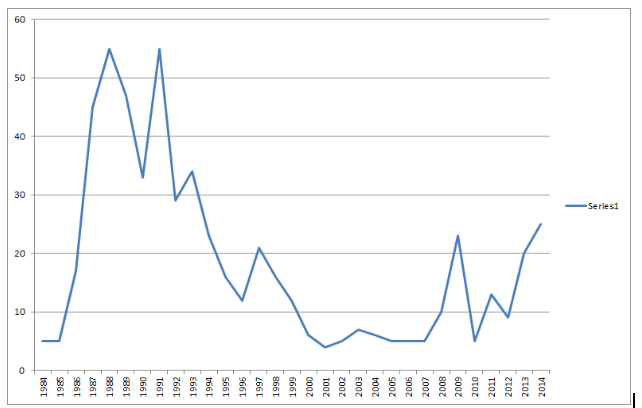
\includegraphics[width=9cm]{figs/citations.png}    
    		\caption{Sum of citations of 11 key papers on cognitive effects of programming 1984-2014. Calculated using Web of Science}
	\end{figure}
	\tiny Source: \textit{Nina Breshnihan, Trinity College Dublin}
\end{center}

\end{frame}

\usebackgroundtemplate{}

%--------------------------------------------------------
%\usebackgroundtemplate{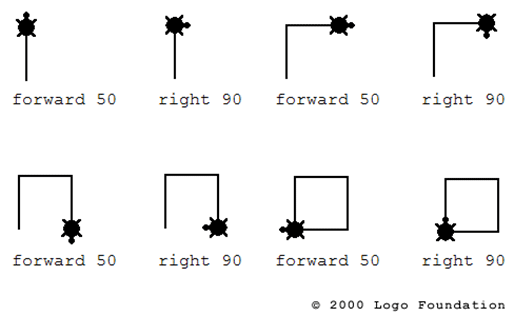
\includegraphics[height=10cm]{figs/turtles.png}}
% background: http://www.wim-network.org/wp-content/uploads/2012/04/iceberg.jpg

\begin{frame}
\frametitle{Code to learn}
\begin{columns}[T]
  \begin{column}{0.5\textwidth}
    \begin{figure}[t!]
      \begin{center}
	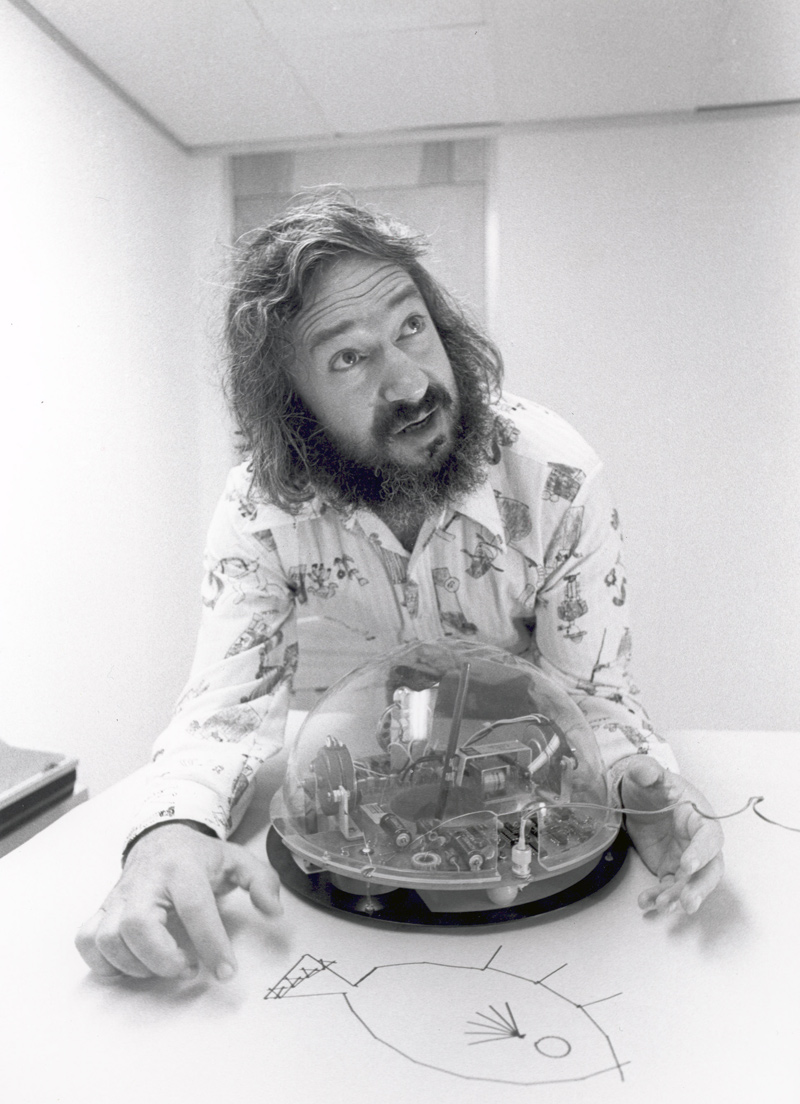
\includegraphics[width=5cm]{figs/seymour.jpg}
      \end{center}
      \label{fig:repetition1}
    \end{figure}
  \end{column}
  \begin{column}{0.5\textwidth}
    \begin{block}{The Logo programming language}
      \begin{itemize}
	 \item Developed in the late 1960s
         \item Its educational impact was intensively investigated in the 70s and 80s
         \item Students' improvements in maths (and other disciplines) were proved
         \item ``Disappeared'' from the educational landscape in the mid-90s
      \end{itemize}
    \end{block}
    \hfill{\Tiny Seymour Papert's picture: jgora.net}
  \end{column}
\end{columns}
\end{frame}


\usebackgroundtemplate{}


%%--------------------------------------------------------

\begin{frame}
\frametitle{History of learning \emph{with} computers}
\begin{center}
	\begin{figure}[t!]
		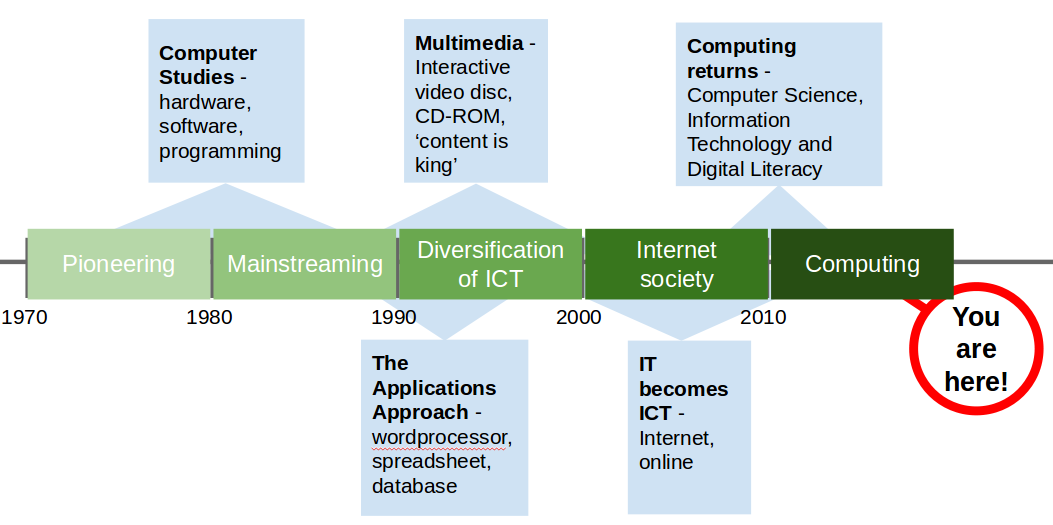
\includegraphics[width=11cm]{figs/history.png}    
    		\caption{You are here!}
	\end{figure}
	\tiny Source: \textit{REaCT EU project proposal}
\end{center}

\end{frame}

\usebackgroundtemplate{}



%%--------------------------------------------------------

\usebackgroundtemplate{
\includegraphics[width=13cm]{figs/future.png}}
%background: https://www.flickr.com/photos/lendingmemo/11746994686

\begin{frame}
\frametitle{About Computational Thinking}


  \begin{center}  
    \LARGE 2. Computational thinking skills can be acquired by other means, but probably programming is the most cost-effective way to do it nowadays
  \end{center}
\vspace{\baselineskip}
\vspace{\baselineskip}
\vspace{1.2cm}
\hfill{\Tiny Background picture: Simon Cunningham }
%
\end{frame}

\usebackgroundtemplate{}


%%--------------------------------------------------------

\usebackgroundtemplate{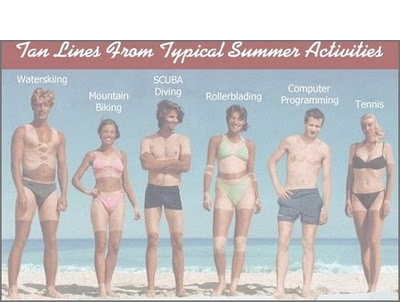
\includegraphics[width=12.2cm]{figs/programming2.png}}
%background: 

\begin{frame}
\frametitle{About Programming}

\vspace{2.7cm}

  \begin{itemize}
    \item Programming is \emph{cheap}
    \item Programming is ubiquitous: it can be done in isolation, and in group... locally or over the Internet
    \item Programming promotes some social skills and team work
    \item Programming practice provides early (usually, instantaneous) feedback
    \item Programming releases endorphins (no scientific evidence, yet ;)
    \item There are (software) tools that can help in the learning process
  \end{itemize}
\vspace{-0.4cm}
\hfill{\Tiny Background picture: (c) Duncan Hill. Flickr}
%
\end{frame}

\usebackgroundtemplate{}


%%--------------------------------------------------------

\usebackgroundtemplate{
\includegraphics[width=13cm]{figs/future.png}}
%background: https://www.flickr.com/photos/lendingmemo/11746994686

\begin{frame}
\frametitle{About Computational Thinking}


  \begin{center}  
    \LARGE 3. Computational thinking skills are not only for STEM (or for learning STEM)
  \end{center}
\vspace{\baselineskip}
\vspace{\baselineskip}

\vspace{2.5cm}
\hfill{\Tiny Background picture: Simon Cunningham }
%
\end{frame}

\usebackgroundtemplate{}

%%--------------------------------------------------------

\usebackgroundtemplate{
\includegraphics[height=8.8cm]{figs/humanities.png}}
%background: 

\begin{frame}
\frametitle{Coding beyond STEM}

  \begin{itemize}
    \item STEM + Art = STEAM. Haven't heard about it before? 
    \item Programming is a way of expression (that is complementary to other ways of expressing yourself)
    \item Learners become \emph{prosumers}, not just consumers of technology
    \item There is (preliminary) research on the (good) effects of coding in other subjects
  \end{itemize}


\vspace{2.5cm}
\hfill{\Tiny Background picture: ngu.edu}
%
\end{frame}

\usebackgroundtemplate{}



%%--------------------------------------------------------

\usebackgroundtemplate{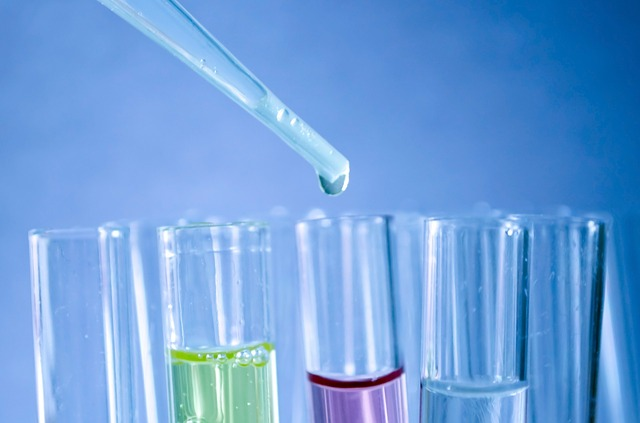
\includegraphics[width=13cm]{figs/research2.jpg}}
% https://pixabay.com/en/test-tube-lab-medical-research-214185/
\begin{frame}
\frametitle{CT Research}


  \begin{center}  
    \LARGE 4. We are performing research on the topic in eMadrid!
  \end{center}
\vspace{\baselineskip}
\vspace{\baselineskip}
\vspace{1.3cm}
\hfill{\Tiny Background picture: Pixabay - Public Domain}
%
\end{frame}

\usebackgroundtemplate{}

%%--------------------------------------------------------

\usebackgroundtemplate{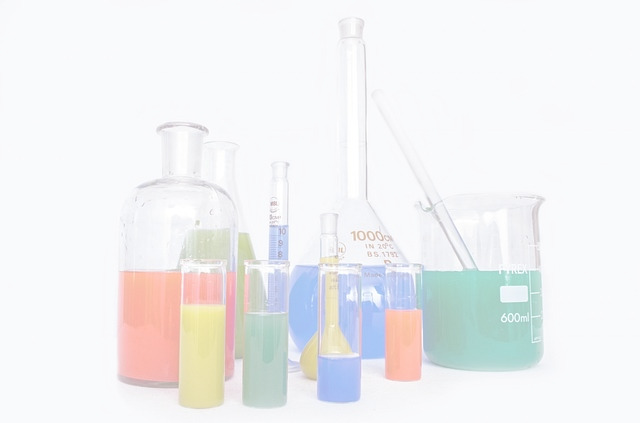
\includegraphics[height=8.8cm]{figs/research.jpg}}
%background: 

\begin{frame}
\frametitle{CT Research @ URJC}

  \begin{itemize}
    \item Assessment of Computational Thinking skills
    \begin{itemize}
      \item Dr.Scratch on-line gamified evaluation tool
      \item Evaluation frameworks (Bebras, TPC...)
    \end{itemize}
    \item Experimentation
    \begin{itemize}
      \item Age (i.e., when do we start?)
      \item Gender (i.e., is the effect the same?)
      \item Subject (i.e., maths \emph{vs.} social sciences?)
      \item Topic (i.e., what skills are developed with different type of programs?)
      \item Unbundling the learning process (i.e., social learning? gamification?)
    \end{itemize}
  \end{itemize} 

\vspace{1.5cm}
\hfill{\Tiny Background picture: Pixabay - Public domain}

\end{frame}

\usebackgroundtemplate{}


%%--------------------------------------------------------
\usebackgroundtemplate{
\includegraphics[width=13cm]{figs/take-away.jpg}}
%% background: http://flamingcow.co.uk/wp-content/uploads/2015/02/takeaway-940x283.jpg

\begin{frame}
\frametitle{In short...}

  \begin{enumerate}
    \item Computation thinking is a \emph{renaming} of something that already occurred in the 70s and 80s and that disappeared in the 90s. Let's not happen that again!
    \item Computational thinking skills can be acquired by other means, but probably programming is the most cost-effective way to do it nowadays
    \item Computational thinking skills are not only for STEM (or for learning STEM)
    \item We are performing research on the topic in eMadrid!
  \end{enumerate}

\vspace{1.5cm}
\hfill{\Tiny Background picture: flamingcow.co.uk}
%
\end{frame}

\usebackgroundtemplate{}

%--------------------------------------------------------
\frame{
\maketitle
\begin{center}

\includegraphics[width=2cm]{format/libresoft-logo}
\hspace{0.5cm}

\includegraphics[width=5cm]{format/gsyc-urjc}
\vspace{0.5cm}

\includegraphics[width=3cm]{format/emadrid.png}
\end{center}
}

\end{document}
